\section*{Implementation}
\addcontentsline{toc}{section}{Implementation}
To allow for interactions and an evaluation of the whole design, an interactive prototype is advantageous. The prototype developed throughout the concept phase of the project needed to be implemented using Axure RP 10, a commercial prototyping tool with many benefits and drawbacks.

The design was split up into different components to increase modularity and allow multiple people to work on the prototype simultaneously. This way, changes in the design of the component “slider” get applied to all instances automatically. The drawback is, that we cannot get the position of a single slider as a variable. When dragging any of the three sliders, the values of all three got overwritten. The issue was resolved by utilizing external objects that observe their position. Instead of the sliders setting the variable themselves, these observing objects monitor the position of them externally and set the values for them. These workarounds had to be used throughout the whole prototyping phase of the project, as Axures “Interactions”-feature is far from polished. 

\begin{figure*}[htp]
    \centering
    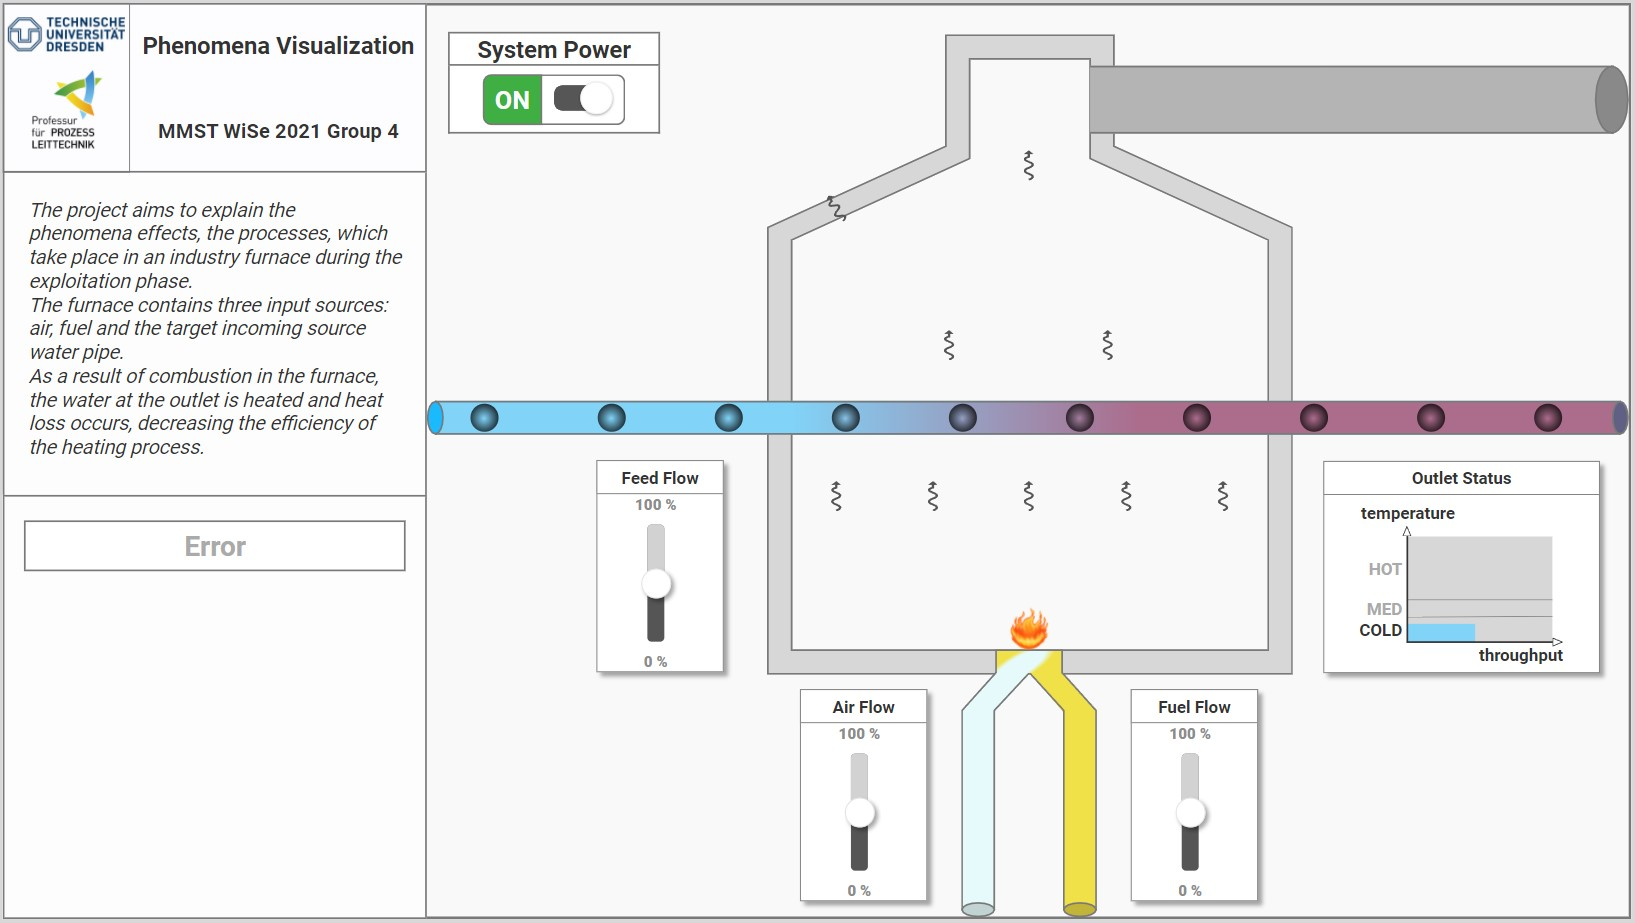
\includegraphics[width=1\linewidth]{images/concept/prototype/prototype_final.jpg}
    \caption{final prototype with animations, using a fire animation \cite{davin_fireball_2021}}
\label{fig:axure_final_prototype}
\end{figure*}

The values of the sliders reach from zero to one and are used for the different functions in the prototype. The combustion function is the product of the air and fuel values. By multiplying them, the function stays zero if either one of them is turned off and reaches its maximum if both are set to their maximal values. As this phenomena visualization should not be based on real physical formulas, the result gets linearized between zero and one and stored in a “combustion”-variable. This value is used for changing the size of the flame animation and corrugated arrows as well as the color of the exhaust pipe. In Axure, color is a property of every element and can either be set through \ac{HEX} or \ac{RGB} values. Unfortunately, neither one of them can updated during runtime and the color cannot be changed automatically. To still be able to display the change in color of the exhaust, a dark-grey exhaust pipe was placed on top of a light-grey pipe. By adapting the opacity of the dark-grey component on top according to the value of the “combustion”-variable, a continuous change in color can be achieved. The same method was used to display the gradient in temperature of the feed flow.

The feed flow is visualized as a stream of “bubbles” moving continuously from left to right. Their speed changes according to the slider position. Whenever a bubble reaches the end of the pipe it moves back to the beginning. These ten moving elements max out the performance capacity of Axure and introduced different artifacts like bubbles disappearing randomly or jittering arrows. After utilizing very unconventional methods, like making bubbles wait for 0.5 seconds invisibly after moving them back to relieve the scheduler, the prototype was running smoothly.

\begin{figure*}[htp]
    \centering
    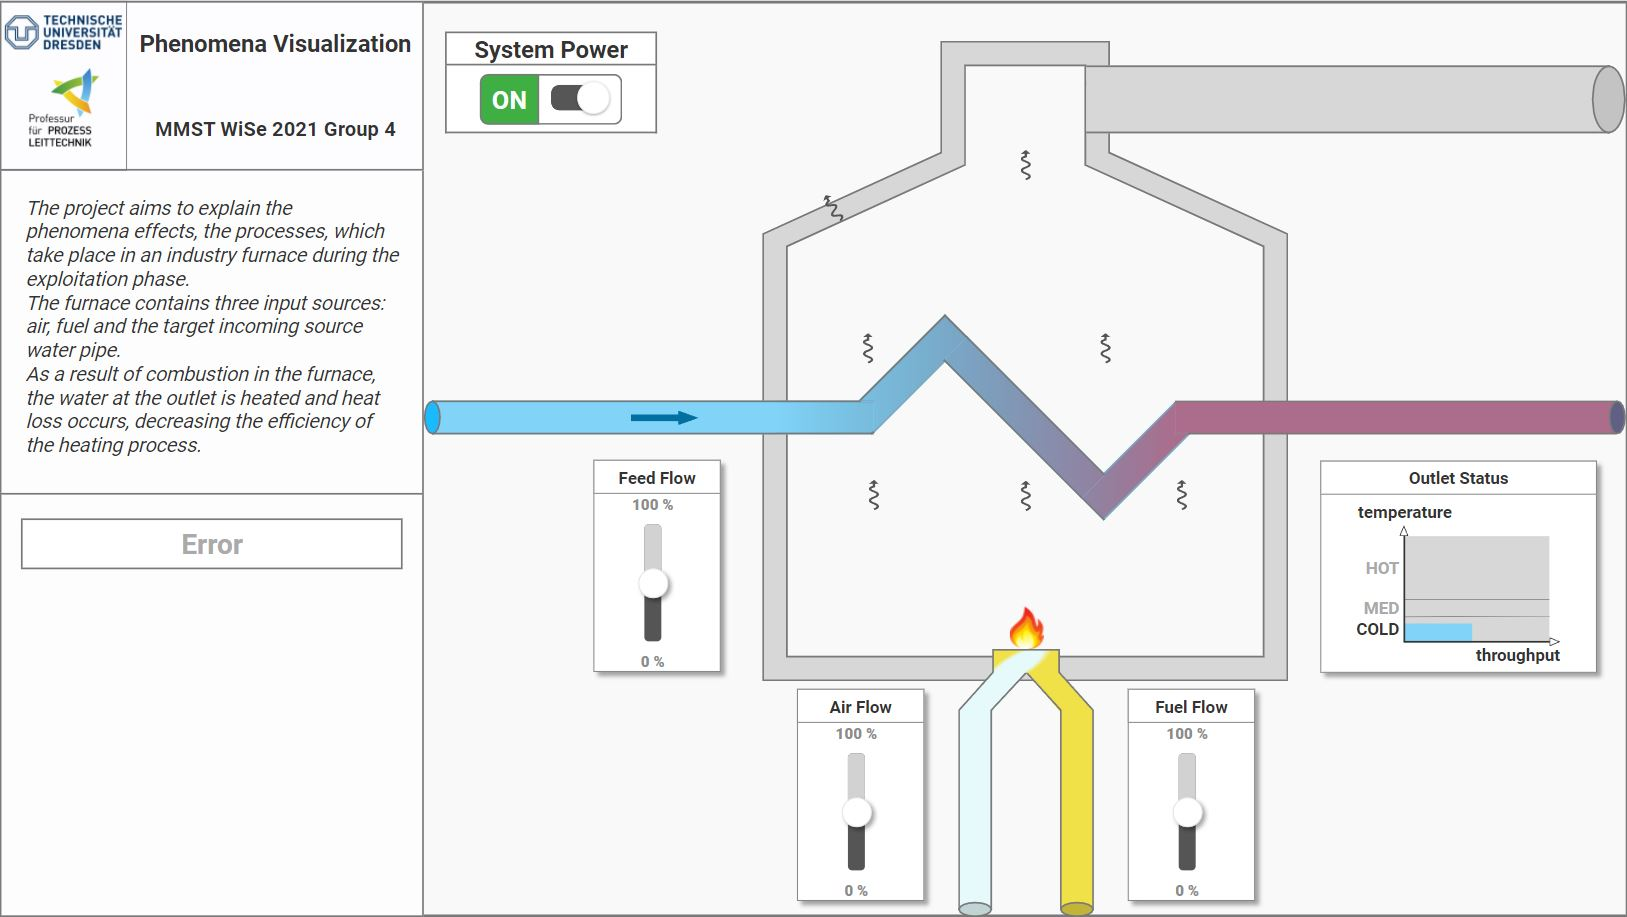
\includegraphics[width=1\linewidth]{images/concept/prototype/prototype_final_woAnimation.JPG}
    \caption{final prototype without animations, using a static flame \cite{john3_free_fire_2019}}
\label{fig:axure_final_prototype_wo_animations}
\end{figure*}

The creation process of an \ac{HMI} is always about comparing different design options and choosing the best-suited for the application. This assessment is subjective, and many options have benefits and drawbacks. For the prototype of the furnace visualization, animations for the fire and feed flow have been implemented to draw attention and raise user awareness. To implement them with Axure, the feed pipe needed to be straight, which could convey a wrong message as most furnaces use winded pipes to transfer as much heat into the feed as possible. A second prototype as shown in figure \ref{fig:axure_final_prototype_wo_animations} was implemented to visualize that, but this would not allow for the animations to be implemented. In the final product, the best of both designs could be realized, but this was not feasible with Axure.

